\documentclass[12pt, a4paper]{scrreprt}

\usepackage{mystyle}
\usepackage{graphicx}

\begin{document}

\pagenumbering{Roman}
\newgeometry{margin=1.5cm}
\begin{titlepage}

  \includesvg[width=0.25\textwidth]{Grafiken/LogoHS_Esslingen}\\ \vspace{3cm}
  
  \begin{center}
    {\usekomafont{disposition}
      \Huge Formelsammlung Physik 2}
    \vspace{0.5cm}
    
    \begin{Large}
      Tim Hilt\\
      \vspace{0.4cm}
      \today\\
    \end{Large}
    
  \end{center}
\end{titlepage}
\restoregeometry

%%% Local Variables:
%%% mode: latex
%%% TeX-master: "Physik2Formelsammlung"
%%% End:

\tableofcontents
\listoffigures
\newpage
\linespread{1.5} % Nicht in der Präambel sondern nach dem Inhaltsverzeichnis, da dieses sonst sehr in die Länge gezogen wird

\pagenumbering{arabic}
%------------------------ Schwingungen -----------------------

\chapter{Schwingungen}

\section{Dummy}
Dies ist eine Dummy-Section und ich werde sie nicht benutzen.

\section{Formelzeichen}

\begin{center}
  \makegapedcells
  \begin{tabular}{l | l | r}
    Formelzeichen & Physikalische Größe & Einheit\\
    \hline \hline
    \(f\) & Frequenz & Hz\\ \hline
    \(T\) & Schwingungsdauer & \(s\)\\ \hline
    \(\omega _0\) & Winkelgeschwindigkeit (ungedämpftes System) & \(s^{-1}\)\\ \hline
    \(\omega _d\) & Winkelgeschwindigkeit (gedämpftes System) & \(s^{-1}\)\\ \hline
    \(k\) & Federkonstante & \(\frac{N}{m}\)\\ \hline
    \(x\) & Auslenkung & \(m\)\\ \hline
    \(D\) & Dämpfungskonstante & (Einheitenlos)\\ \hline
    \(\delta\) & Abklingkoeffizient & \(s^{-1}\)\\ \hline
    \(b\) & Reibkonstante & \(\frac{kg}{s}\)\\ \hline
    \(F_E\) & Anregende Kraft & \(N\)\\ \hline
    \(E_v/E_n\) & Energie davor / Energie danach\\ \hline
    \(J\) & Massenträgheitsmoment & \(kg*m^2\)\\ \hline
    \(\varphi\) & Drehwinkel & Bogenmaß\\ \hline
    \(M\) & Drehmoment & \(Nm\)\\ \hline
  \end{tabular}
\end{center}


\section{Formeln}


\subsection{Allgemein}

\paragraph{\(k_{Ges}\), wenn Federn parallel} \dotfill \(k_{Ges}=k_1+k_2+k_3+ \dots +k_n\)
\paragraph{\(k_{Ges}\), wenn Federn seriell} \dotfill \(\frac{1}{k_{Ges}}=\frac{1}{k_1}+\frac{1}{k_2}+\frac{1}{k_3}+ \dots +\frac{1}{k_n}\)
\paragraph{Eigenkreisfrequenz} \dotfill \(\omega=2\pi*f=\frac{2\pi}{T}\)
\paragraph{Umrechnung \(f\) / \(T\)}\dotfill \(f=\frac{1}{T}\); \(T=\frac{1}{f}\)
\paragraph{Allgemeine Schwingungsdgl} \dotfill \(m* \ddot x + b*\dot x + k *x=F_E\)
\paragraph{Drehmoment} \dotfill \(M = k * J = F * x\) (wobei x die Länge des Hebelarms darstellt)


\subsection{Ungedämpfte Systeme}

\paragraph{Kriterium für harmonische Schwingung: } \mytextred{\(\frac{x}{F}\), bzw. \(\frac{\varphi}{M}\) muss linear sein!}
\paragraph{Weg-Zeit-Funktion ungedämpfter Systeme} \dotfill \(x(t)=x_m* \cos(\omega t + \varphi_0)\)
\paragraph{Schwingungsdauer ungedämpft} \dotfill \(T_0=2\pi*\sqrt{\frac{m}{k}}\)
\paragraph{Maximale Geschwindigkeit im Schwingvorgang} \dotfill \(y_{\max} = x_m * \omega _0\)\\
\myhspace \textcolor{myred}{\(v_{\min}\) ist immer \(= 0\)!}
\paragraph{Amplitude \(x_m\)} \dotfill \(x_m = \sqrt{x_0^2 + {\left( \frac{v_0}{\omega _0} \right)}^2}\)
\paragraph{Kreisfrequenz ungedämpft} \dotfill \(\omega_0=\sqrt{\frac{k}{m}}\) Und bei Drehbewegungen: \(\omega_0=\sqrt{\frac{k}{J}}\)
\paragraph{Hookesches Gesetz} \dotfill \(F_s=k*x\)
\paragraph{Hookesches Gesetz bei Drehbewegungen} \dotfill \(M = k * \varphi\)

\subsubsection{U-Rohr}
\paragraph{Schwingungsdgl am U-Rohr} \dotfill \(\underbrace{\rho*A*l}_\text{m}*\ddot x+\underbrace{\rho*A*g*2}_\text{k}x=0\)\\
(\(x=x_0*\cos(\omega_0*t)\))


\subsection{Gedämpfte Systeme}

\paragraph{Abklingfunktion} \dotfill \(x_m=x_0*e^{-\delta*t}\)
\paragraph{Kreisfrequenz gedämpft} \dotfill \(\omega_d=\sqrt{\omega_0^2-\delta^2}=\omega_0\sqrt{1-D^2}\)
\paragraph{Abklingkoeffizient} \dotfill \(\delta=\frac{b}{2m}=D*\omega_0\)
\paragraph{Dämpfungskonstante} \dotfill \(D=\frac{\delta}{\omega_0}\)
\paragraph{Schwingungszeit gedämpft} \dotfill \(T_D=\frac{2\pi}{\sqrt{\omega_0^2-\delta^2}}=\frac{T_0}{\sqrt{1-D^2}}\)
\paragraph{Reibkonstante} \dotfill \(b=\delta * 2m\)
\paragraph{Logarithmisches Dekrement} \dotfill \(\Lambda=\delta*T_0\)
\paragraph{Güte} \dotfill \(Q=\frac{\pi}{\delta*T}=\frac{1}{2D}\)
\paragraph{Schwingungsenergie} \dotfill \(E = \frac{1}{2}*c*x^2\)
\paragraph{Energieverlust} \dotfill
\(\frac{\Delta E}{E} = 1-\frac{E_n}{E_v}=1-\frac{\frac{1}{2}\ c\ x_1^2}{\frac{1}{2}\ c\ x_0^2}\)\\
\-\hspace{1.5cm}Kann noch gekürzt werden! \dotfill \(1-\frac{x_1^2}{x_0^2}\)

\subsubsection{Aperiodischer Grenzfall}
\(D=1\)\\
\(\delta=\omega_0\)\\
\(b=2m*\omega_0\)


\subsection{Erzwungen schwingende Systeme}


%------------------------ Akustik --------------------------
\chapter{Akustik}

\section{Formelzeichen}

\begin{center}
  \makegapedcells{}
  \begin{tabular}{l l r}
    Formelzeichen & Physikalische Größe & Einheit\\
    \hline \hline
    \(f\) & Frequenz & \(Hz\)\\ \hline
    \(L\) & Schallpegel & \(dB\)\\ \hline
    \(c\) & Ausbreitungsgeschwindigkeit & \(\frac{m}{s}\)\\ \hline
    \(\lambda\) & Wellenlänge & \(m\)\\ \hline
    \(I\) & Schallintensität & \(\frac{W}{m^2}\)\\ \hline
    \(P\) & Schallleistung & \(W\)\\ \hline
    \(A\) & Oberfläche (Kugelwelle) & \(m^2\)\\ \hline
    \(Z\) & Wellenwiderstand/Schallkennimpedanz & \(\frac{kg}{m^2s}\)\\ \hline
    \(\rho\) & Dichte & \(\frac{kg}{m^3}\)\\ \hline
    \(p\) & Schalldruckamplitude & \(Pa\)\\ \hline
    \(Ma\) & Machzahl & Einheitenlos\\ \hline
  \end{tabular}
\end{center}

\section{Konstanten}
\(I_0 = 10^{-12}\ \frac{W}{m^2}\)

\section{Formeln}
\paragraph{Schallgeschwindigkeit} \dotfill \(c=\lambda * f\)\\
\paragraph{Schallintensitätspegel} \dotfill \(L_I = 10\log \left(\frac{I}{I_0}\right)\)\\
\-\hspace{1.5cm}\textcolor{myred}{Wichtigste Formel für Rechnung mit Schallwellen!}\\
\paragraph{Summe mehrerer \textcolor{myred}{gleich lauter} Schallpegel} \dotfill \(L_{\sum} = 10 \log(n) + L_0\)\\
\-\hspace{1.5cm}, wobei \(n\) die Anzahl der Schallquellen ist und \(L_0\) der Pegel einer einzelnen Schallquelle.

\paragraph{Summe mehrerer \textcolor{myred}{unterschiedlich lauter} Schallquellen} \dotfill \(L_{\sum} = 10 * \log(10^{L_1/10} + 10^{L_2/10} + 10^{L_3/10}+ \cdots + 10^{L_n/10})\)\\[1em]
\myhspace Beispiel:
\begin{align*}
  L_1 &= 90 dB, L_2 = 80 dB, L_3 = 65 dB\\[1.25em]
  L_{\sum} &= 10 * \log(10^9 + 10^8 + 10^{6.5})\\[1em]
  L_{\sum} &= 90.426 dB
\end{align*}


\paragraph{Schallpegeldifferenz:}
%
%
% --------- Rahmt NUR die Formel selbst ein -------------
\begin{empheq}[box=\fbox]{align*}
  \Delta L &= L_2 - L_1 \\
           &= 10 \log \left(\frac{I_2}{I_1}\right)\\
  \text{\footnotesize Und bei unterschiedlichem Radius/Abstand: }\\ &= 20\log \left(\frac{r1}{r2}\right)
\end{empheq}

wobei \textcolor{myred}{\(L_2\) der größere} beider Werte ist\\
\paragraph{Schallintensität} \dotfill \(I = \frac{P}{A} \quad = \frac{\rho * x^2 * \omega^2 * c}{2}\)\\
\begin{framed}
Bei allen fahrenden / mit der Erde verbundenen Schallquellen gilt \mybfred{\(\boldsymbol{A = 2\pi r^2}\)}. Dies entspricht der Oberfläche einer Halbkugel. Dementsprechend gilt für alle fliegenden oder in der Luft aufgehängten Schallquellen \mybfred{\(\boldsymbol{A=4\pi r^2}\)}
\end{framed}
\paragraph{Schallintensität Halbkugel} \dotfill \(I = \frac{P}{2\pi*r^2}\)
\paragraph{Schallintensität Kugel} \dotfill \(I = \frac{P}{4\pi*r^2}\)\\
\-\hspace{1.5cm}z.B bei Aufgabenstellung \glqq{} Geben Sie Intensität in einer Entfernung von (\(r\)) Metern an.\grqq{}
\paragraph{Schallkennimpedanz / Wellenwiderstand} \dotfill \(Z=\rho * c\)
\paragraph{Schalldruckamplitude} \dotfill \(p = Z * \omega * x\)
\paragraph{Umrechnung vom Effektivwert} \dotfill \(p = \sqrt{2} * p_{\mathrm{eff}}\)
\paragraph{Dopplereffekt}

\begin{empheq}[box=\fbox]{align*}
  \text{\footnotesize Ruhender Empfänger, bewegter Sender: } \qquad f_E &= f_S \frac{1}{1 \mp \frac{v_S}{c}}\\[1em]
  \text{\footnotesize Runder Sender, bewegter Empfänger:} \qquad f_E &= f_S \left( 1 \pm \frac{v_E}{c} \right)\\[1em]
  \text{\footnotesize Bewegter Sender, bewegter Empfänger: } \qquad f_E &= f_S \frac{c \pm v_E}{c \mp v_S}\\
\end{empheq}
\-\hspace{1.5cm} \textcolor{myred}{Oberes Zeichen: Annäherung; Unteres Zeichen: Entfernung}

\vspace*{1cm}
\paragraph{Machscher Kegel} \dotfill \(\sin \left( \frac{\alpha}{2} \right) = \frac{c}{v_S} = \frac{1}{Ma}\)
\paragraph{Machzahl} \dotfill \(Ma = \frac{v_S}{c}\)
\paragraph{Ab wann Überschallknall?} \dotfill \(c = v \text{ \footnotesize Bei Drehbewegung: }\frac{c}{r} = \frac{v}{r} = \omega\)





%------------------------- Wellen ----------------------------
\chapter{Wellen}

\section{Formelzeichen}
\(\lambda=\) \dotfill Wellenlänge\\
Umrechung von Bogensekunden in Grad: \dotfill \(0 \degree 0\degree \text{Wert}\degree\) Danach ist Wert für weitere Berechnungen nutzbar

\section{Formeln}

\chapter{Stehende Wellen}

\section{Formelzeichen}

\begin{center}
  \makegapedcells{}
  \begin{tabular}{l | l | r}
    Formelzeichen & Physikalische Größe & Einheit\\\hline \hline
    \(\lambda\) & Wellenlänge & \(m\)\\ \hline
    \(\rho\) & Dichte & \(\frac{kg}{m^3}\)\\ \hline
    \(f\) & Frequenz & \(Hz\)\\ \hline
    \(l\) & Länge & \(m\)\\ \hline
    \(k\) & Anzahl d. Wellenbäuche & Wellen/m\\ \hline
    \(p\) & Luftdruck & \(Pa\)\\ \hline
    \(\kappa\) & Isentropenexponent; \(\frac{c_p}{c_v}\) & Einheitenlos\\ \hline
  \end{tabular}
\end{center}

\section{Konstanten}
\mytextred{Menschlicher Hörbereich:} \(16 - 20000 Hz\)\\

\section{Formeln}
\paragraph{Schallgeschwindigkeit} \dotfill \(c = \sqrt{\frac{\kappa * p}{\rho_T}} = 331\frac{m}{s} * \sqrt{\frac{273K + \cdots \degree C}{273K}}\)
\paragraph{Länge der Saite/des Rohres (gleiche Enden)} \dotfill \(l = (k + 1) * \frac{\lambda}{2} = (k + 1) * \frac{c}{2f}\)\\
\myhspace \mytextred{\(k \in 0, 1, 2, \dots\)}
\paragraph{Länge der Saite/ des Rohres (ungleiche Enden)} \dotfill \(l = (2k+1) * \frac{\lambda}{4} = (2k+1) * \frac{c}{4f}\)\\
\myhspace \mytextred{\(k \in 0, 1, 2, \dots\)}\\
\myhspace \mytextred{\glqq{} 1. Harmonische\grqq{} \(\equiv\) \glqq{} Grundschwingung \grqq{} \(\equiv\) \glqq{} 0. Oberschwingung\grqq{}}
\paragraph{Länge einfachster Fall (gleiche Enden)} \dotfill \(l = \frac{\lambda}{2} = \frac{c}{2f_0}\)\\
\myhspace \mytextred{Gilt nur für Grundschwingung!}
\paragraph{Länge einfachster Fall (ungleiche Enden)} \dotfill \(l = \frac{\lambda}{4} = \frac{c}{4f_0}\)\\
\myhspace \mytextred{Gilt nur für Grundschwingung!}
\paragraph{Grundschwingung/Wellenlänge gleiche Enden} \dotfill \(f = \frac{c}{4*l} ; \lambda = 4 * L\)
\paragraph{Grundschwingung ungleiche Enden} \dotfill \(f = \frac{c}{2*l} ; \lambda = 2 * L\)
\paragraph{Frequenzverhältnis} \dotfill Bsp. \(\frac{5}{4} \rightarrow \frac{\text{Frequenz nachher}}{\text{Frequenz vorher}}\)
\paragraph{Wellenzahl} \dotfill \(k = \frac{2\pi}{\lambda} = \frac{\omega}{c}\)
\paragraph{Wellengeschwindigkeit} \dotfill \(c = \sqrt{\frac{F_G}{\rho * A}}\) bzw. \(= \sqrt{\frac{F(x)_G}{\rho * A}}\)\\ , Wenn nicht die gesamte, sondern die Geschwindigkeit an einer bestimmten Stelle gesucht ist



%-------------------------- Optik ---------------------------
\chapter{Optik}

\section{Formelzeichen}

\begin{center}
  \makegapedcells
  \begin{tabular}{l | l | r}
    Formelzeichen & Physikalische Größe & Einheit\\
    \hline \hline
    \(\lambda\) & Wellenlänge & \(m\)\\ \hline
    \(c\) & Lichtgeschwindigkeit & \(\frac{m}{s}\)\\ \hline
    \(f\) & Frequenz & \(Hz\)\\ \hline
    \(R\) & Reflexionsgrad & Gibt reflektierten Anteil\\ \hline
    \(T\) & Transmissionsgrad & Gibt transmittierten Anteil\\ \hline
  \end{tabular}
\end{center}

\section{Konstanten}
\(c_0 = 3*10^8\frac{m}{s}\)\\[1em]
\textcolor{myred}{Wellenlängenempfindlichkeit des Auges:} \(400 - 750\ nm\)\\

\begin{figure}[H]
  \centering
  \includesvg[width = \textwidth]{Grafiken/Farbspektrum}
  \caption[Farbspektrum]{Farbspektrum und menschlicher Sehbereich}
  \label{fig:Spektrum}
\end{figure}

\section{Formeln}
\paragraph{Zusammenhang Frequenz / Ausbreitungsgeschwindigkeit} \dotfill \(c = f * \lambda\)
\paragraph{Abstand berechnen (Radarpistole u.Ä.)} \dotfill \(s = \frac{c * t}{2}\)\\
\myhspace \textcolor{myred}{Aus Formel der Kinetik \(v = \frac{s}{t}\)}
\paragraph{Frequenzverschiebung} \dotfill \(\Delta f = \frac{2 * f_s * v}{c} = \frac{2 * v}{\lambda_s}\)
\paragraph{Geschwindigkeit Zielfahrzeug} \dotfill \(v = \frac{\Delta f * \lambda_s}{2} = c * \left( \frac{\Delta f}{f_R'+f_R} \right) \)\\
\myhspace\textcolor{myred}{Wenn beide Objekte sich bewegen ist \(v = \Delta v\)}

\subsection*{Frequenzverschiebung beim Dopplereffekt}
\addcontentsline{toc}{subsection}{Frequenzverschiebung beim Dopplereffekt}

\begin{framed}
  \textcolor{myred}{
    \begin{tabular}[h]{lclcl}
    Annäherung & $\rightarrow$ & höhere Frequenz / kleinere Wellenlänge & $\rightarrow$ & Violett-Verschiebung\\ 
    Entfernung & $\rightarrow$ & niedrigere Frequenz / größere Wellenlänge & $\rightarrow$ & Rot-Verschiebung
    \end{tabular}
  }
\end{framed}

\paragraph{Optischer Dopplereffekt} \dotfill \(f_E = f_S* \sqrt{\frac{c \pm v}{c \mp v}}\)
\paragraph{Violett- / Rotverschiebung} \dotfill \(\lambda_E = \lambda_S*\sqrt{\frac{1 \mp \frac{v}{c}}{1 \pm \frac{v}{c}}}\)\\
\myhspace{} \textcolor{myred}{Oberes Zeichen: Annäherung; Unteres Zeichen: Entfernung}
\paragraph{Reflexionsgrad \(R\)} \dotfill \(R = {\left( \frac{n_1 - n_2}{n_1 + n_2} \right)}^2\)
\paragraph{Transmissionsgrad \(T\)} \dotfill \(T = 1 - R = \frac{4 n_1 n_2}{{(n_1 + n_2)}^2}\)\\
\myhspace{} Gibt jeweils nur \textbf{einen} Übergang an!\\
\myhspace{} Falls Medium nicht transparent gilt mit dieser Formel der \textbf{Absorptionsgrad}
\paragraph{Transmissionsgrad \textbf{durch} Medium} \dotfill \(T_{Ges} = {(1 - R)}^2 \quad = \quad T_1 \cdot T_2\)


\subsection{Entspiegelung}
Hierbei sei \mytextred{\(n_1 / \lambda_1\)} die Wellenlänge und Brechzahl \mytextred{in Luft}, \mytextred{\(n_2 / \lambda_2\)} die Brechzahl und Wellenlänge \mytextred{in der Entspiegelungsschicht} der Dicke \(d\) und \mytextred{\(n_3 / \lambda_3\)} die Wellenlänge und Brechzahl \mytextred{des Brillenglases}.

\begin{figure}[H]
  \centering
  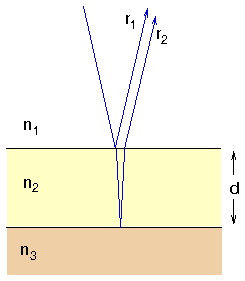
\includegraphics[width = 0.3\textwidth]{./Grafiken/Entspiegelung.png}
  \caption[Entspiegelung]{Grafik zur Veranschaulichung der Entspiegelung}
  \label{fig:Entspiegelung}
\end{figure}

\paragraph{Brechungsindex von Entspiegelungsschicht} \dotfill \(n_2 = \sqrt{n_1 * n_3}\)
\paragraph{Gangunterschied zwischen den beiden Schichten} \dotfill \(\Delta x = 2 * n_2 * d\)
\paragraph{Schichtdicke \(d\)} \dotfill \(d = \frac{\lambda_1}{4n_2}\)


\subsection{Brechung}

\paragraph{Umrechnungen} \dotfill \(\frac{\sin \alpha}{\sin \beta} = \frac{n_2}{n_1} = \frac{c_1}{c_2} = \frac{\lambda_1}{\lambda_2}\)\\
\myhspace{} \mytextred{Von dünn nach dicht $\rightarrow$ zum Lot hin; von dicht nach dünn $\rightarrow$ vom Lot weg}
\paragraph{Ausbreitungsgeschwindigkeit im Medium} \dotfill \(c_n = \frac{c_0}{n}\)
\paragraph{Grenzwinkel der Totalreflexion} \dotfill \(\sin \alpha = \frac{n_1}{n_2}\)\\
\myhspace{} Von dichtem nach dünnem Medium
\paragraph{Brewsterwinkel} \dotfill \(\tan \alpha = \frac{n_2}{n_1}\)\\
\myhspace{} Gilt jeweils, wenn vollständig polarisierter Winkel gefragt ist\\
\myhspace{} \mytextred{\(90 \degree\) zwischen reflektiertem und gebrochenem Strahl}\\
\myhspace{} \mytextred{Der reflektierte Strahl ist vollständig linear polarisiert, der transmittierte Anteil wird vorwiegend parallel polarisiert.}



\end{document}

%%% TeX-command-extra-options: "-shell-escape"
%%% Local Variables:
%%% mode: latex
%%% TeX-master: t
%%% End:
